\subsection*{Problema 37}
\textbf{Enunciado:} Calcular la integral:
\begin{align*}
\int \dfrac{5x^3 + 2}{x^3 - 5x^2 + 4x} \, dx
\end{align*}

\textbf{Solución:} 
Dado que el grado del numerador es igual al grado del denominador, realizamos la división polinómica de la función integrando:
\begin{align*}
\dfrac{5x^3 + 2}{x^3 - 5x^2 + 4x} = 5 + \dfrac{25x^2 - 20x + 2}{x^3 - 5x^2 + 4x}
\end{align*}

El denominador se factoriza como:
\begin{align*}
x^3 - 5x^2 + 4x = x(x - 1)(x - 4)
\end{align*}

Aplicamos fracciones parciales a la parte racional restante:
\begin{align*}
\dfrac{25x^2 - 20x + 2}{x(x - 1)(x - 4)} = \dfrac{A}{x} + \dfrac{B}{x - 1} + \dfrac{C}{x - 4}
\end{align*}

Multiplicando por el denominador común:
\begin{align*}
25x^2 - 20x + 2 &= A(x-1)(x-4) \\
&\quad + Bx(x-4) + Cx(x-1)
\end{align*}

Evaluando en valores convenientes de $x$:
\begin{align*}
x = 0 &\implies 2 = 4A \implies A = \dfrac{1}{2} \\
x = 1 &\implies 7 = -3B \implies B = -\dfrac{7}{3} \\
x = 4 &\implies 322 = 12C \implies C = \dfrac{161}{6}
\end{align*}

Sustituyendo los valores hallados y el cociente de la división en la integral original:
\begin{align*}
\int &\left( 5 + \dfrac{1/2}{x} - \dfrac{7/3}{x - 1} + \dfrac{161/6}{x - 4} \right) dx
\end{align*}

Integramos cada término por separado:
\begin{align*}
&= 5x + \dfrac{1}{2}\ln|x| - \dfrac{7}{3}\ln|x - 1| \\
&\quad + \dfrac{161}{6}\ln|x - 4| + C
\end{align*}

\begin{figure}[H]
	\centering
	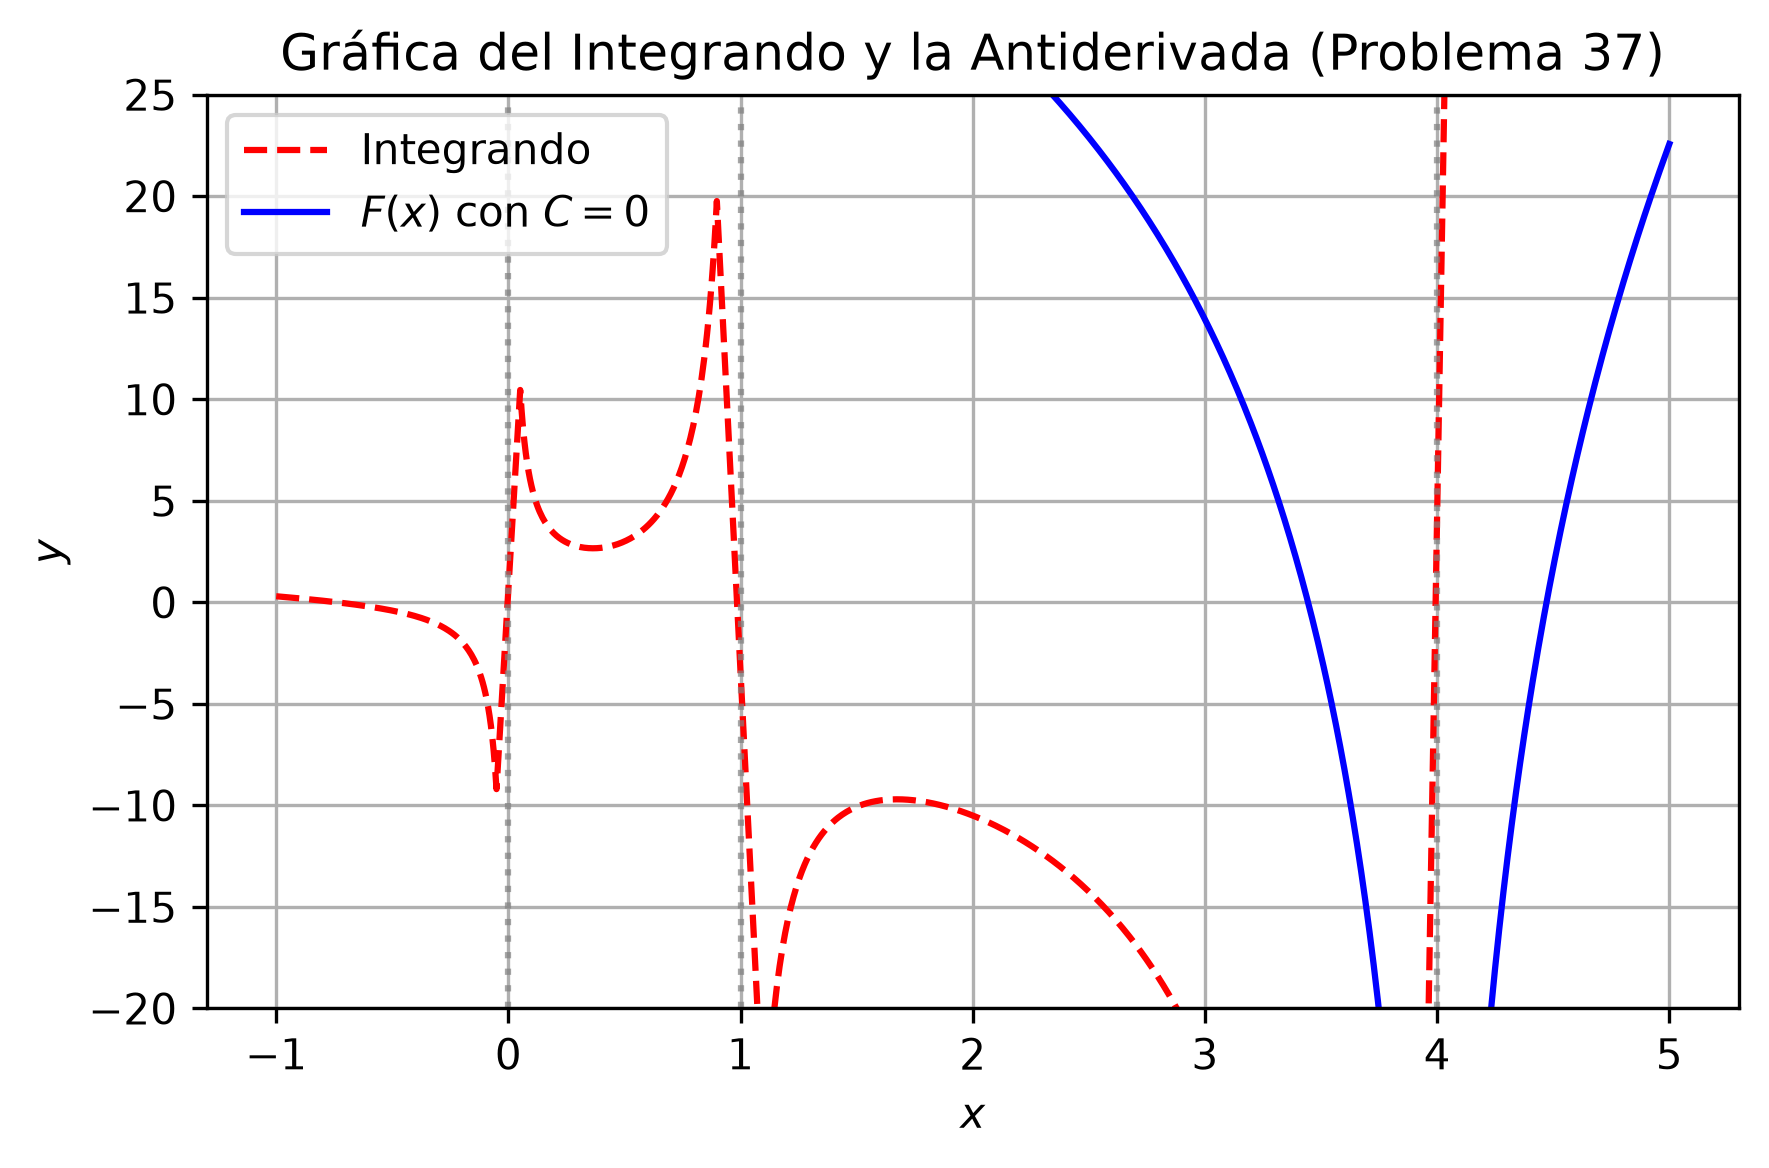
\includegraphics[width=\columnwidth]{semana_03/graficas/SEM03_P37_grafica.png}
	\caption{Representación gráfica de $f(x)$ y su antiderivada $F(x)$ evaluada para la constante de integración $C = 0$ (Problema 37).}
	\label{fig:problema37}
\end{figure}
